\documentclass{article}
\usepackage{tikz}
\usetikzlibrary{arrows,positioning,shapes,fit,calc}

\pgfdeclarelayer{background}
\pgfsetlayers{background,main}

\begin{document}

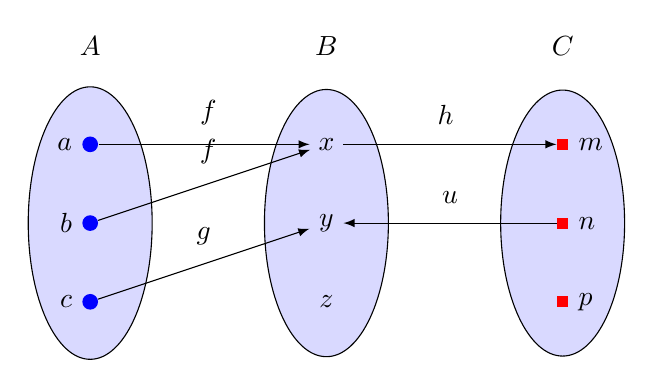
\begin{tikzpicture}[
  every node/.style={on grid},
  setA/.style={fill=blue,circle,inner sep=2pt},
  setC/.style={fill=red,rectangle,inner sep=2pt},
  every fit/.style={draw,fill=blue!15,ellipse,text width=25pt},
  >=latex
]

% set A
\node[setA,label=left:$a$] (a) {};
\node [setA,below = of a,label=left:$b$] (b) {};
\node [setA,below = of b,label=left:$c$] (c) {};
\node[above=of a,anchor=south] {$A$};

% set B
\node[inner sep=0pt,right=3cm of a] (x) {$x$};
\node[below = of x] (y) {$y$};
\node[inner sep=0pt,below = of y] (z) {$z$};
\node[above=of x,anchor=south] {$B$};

% set C
\node[setC,label=right:$m$,right = 3cm of x] (m) {};
\node[setC,label=right:$n$,below = of m] (n) {};
\node[setC,label=right:$p$,below = of n] (p) {};
\node[above=of m,anchor=south] {$C$};

% the arrows
\draw[->,shorten >= 3pt] (a) -- node[label=above:$f$] {} (x);
\draw[->,shorten >= 3pt] (b) -- node[label=above:$f$] {} (x);
\draw[->] (c) -- node[label=above:$g$] {} (y);
\draw[->,shorten <= 3pt] (x) -- node[label=above:$h$] {} (m);
\draw[->] (n) -- node[label=above:$u$] {} (y);

% the boxes around the sets
\begin{pgfonlayer}{background}
\node[fit= (a)  (c) ] {};
\node[fit= (x) (z) ] {};
\node[fit= (m) (p)] {};
\end{pgfonlayer}
\end{tikzpicture}

\end{document}